\chapter{Praktická část}

\section{Metodika}
Z dostupných zdrojů byla nejdříve zjištěna podstata pokusu a~postup jeho provedení. Pokus byl proveden, přičemž byl zdokumentován (fotoaparátem či kamerou) každý krok za účelem možného doplnění nebo opravení nedostatků v~původním zdroji. V~případě potřeby byl pokus zopakován. Zároveň byly poznamenány všechny bezpečnostní požadavky, které vyžadovalo provedení pokusů.

Fotky a~videa byly následně zpracovány dle potřeby do shrnujícího doprovodného videa, nebo jen do souboru doprovodných fotografií. Spolu s~doplněným popisem a~postupem pokusu bylo vše nahráno na stránku \uv{Chemické pokusy} na portálu \uv{WikiKnihy} (\url{https://cs.wikibooks.org/wiki/Chemick%C3%A9_pokusy}) do článku příslušného pokusu. Tato možnost byla zvolena kvůli tomu, že je na internetu a~tedy jednoduše přístupná, dále pro svou otevřenost stejně jako u~jiných \uv{wiki projektů} -- v~případě chyby nebo nepřesnosti může kdokoliv texty jednoduše bez dlouhého kontaktování správců stránky opravit nebo doplnit, jednoduše také může katalog rozšířit. WikiKnihy je projekt celosvětový, pomocí překladů do jiných jazyků se katalog může dostat k~ještě většímu počtu lidí. Licencování obsahu podle Creative Commons též umožňuje používaní obsahu bez problémů s~autorským právem.

\section{Zpracované pokusy}
\subsection{Žíhání skalice}

\B{Zařazení do výuky}

Tento pokus by mohl být zařazen při výuce hydrátů a jejich názvosloví nebo při výuce zkoušky plamenem jako analytické metody. Pokus může být také použit jako podklad pro příklad na výpočet reálného látkového množství nebo hmotnosti odpařené vody nebo zbylého bezvodého síranu v porovnání s jejich teoretickými hodnotami.\\

\hspace{-21pt} \B{Bezpečnost}

Při tomto pokusu se manipuluje s~otevřeným ohněm.\\

\hspace{-21pt} \B{Popis}

Řada solí s~krystalicky vázanou vodou, tzv. hydráty, jsou barevné (zpravidla díky přítomným aquakomplexům kationtů). Barva modré skalice je způsobena přítomností koordinačního kationtu. Při žíhání se modrá skalice zbavuje vázaných molekul vody a~přechází na bílý bezvodý síran měďnatý.\\

Rovnice reakce: \ce{CuSO4 . 5H2O -> CuSO4 + 5H2O }\\

\hspace{-21pt} \B{Postup}

\begin{enumerate}
  \item Sestavíme žíhací aparaturu: na trojnožku umístíme triangl a~pod něj plynový kahan.
  \item V~suché třecí misce rozetřeme asi 1,5 g pentahydrátu síranu měďnatého.
  \item Zvážíme čistý a~suchý žíhací kelímek a~poté do něj nasypeme rozetřený pentahydrát síranu měďnatého (přesné navážky zaznamenáme).
  \item Žíhací kelímek umístíme pomocí laboratorních kleští do trianglu a~žíháme, dokud se zbarvení žíhané látky nezmění z~modré na bílou.
  \item Kelímek necháme zchladnout, zvážíme jej a~z rozdílů hmotnosti před a~po žíhání vypočítáme obsah krystalové vody.
  \item Bezvodý síran měďnatý můžeme pozorovat vlivem vzdušné vlhkosti měnit zabarvení zpátky na modrou.
\end{enumerate}

\begin{figure}[h]
    \centering
    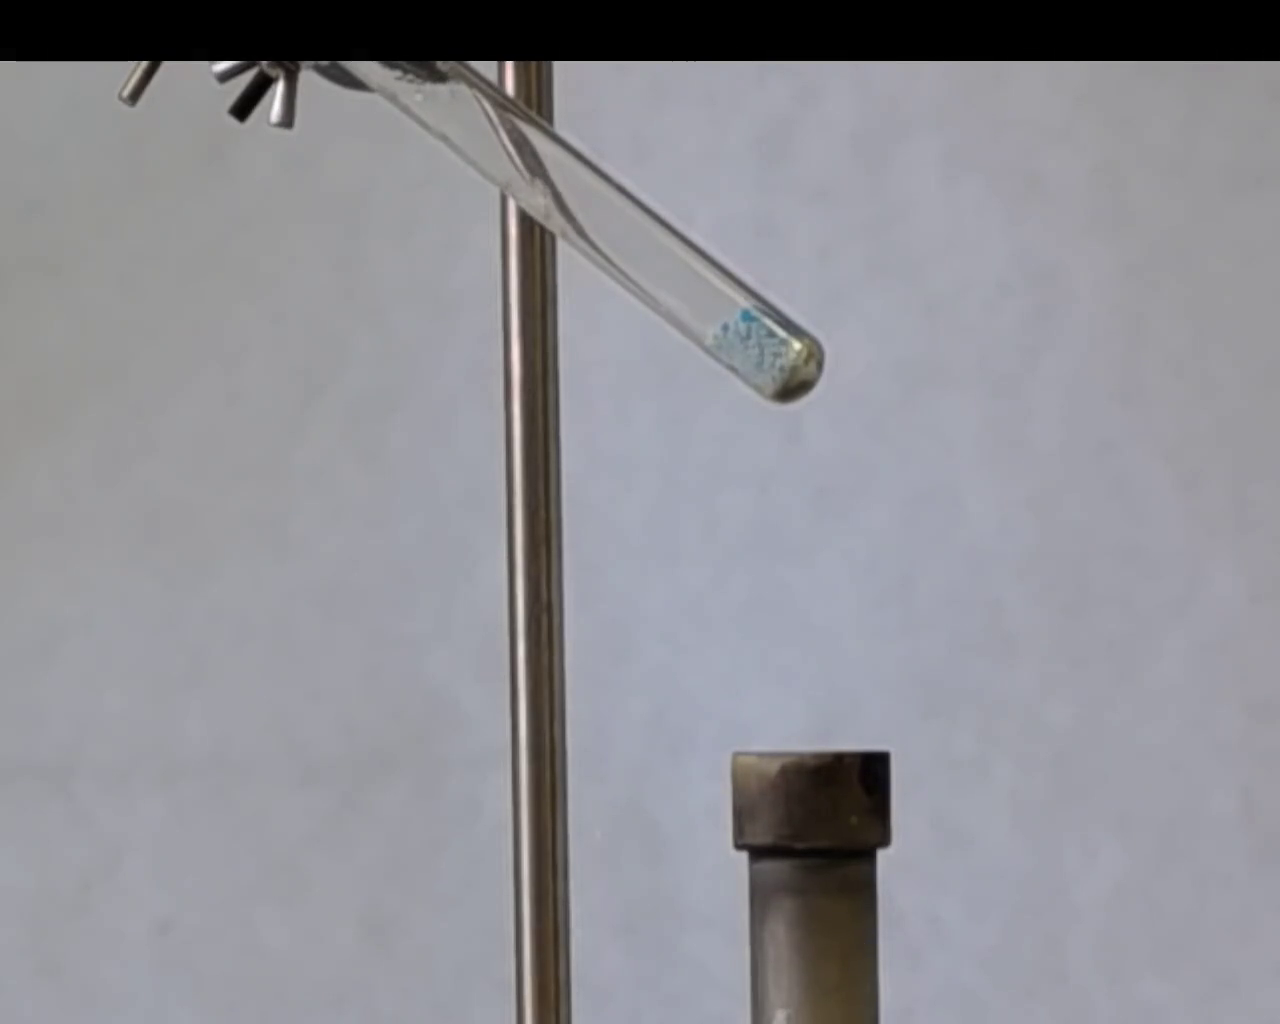
\includegraphics[width=0.45\linewidth]{zihana_skalice.png}
    \caption{Skalice se ztrátou vody ztrácí i barvu}
\end{figure}

\subsection{Zlatý déšť}

\B{Zařazení do výuky}

Tento pokus by mohl být zařazen při výuce srážení jako separační metody nebo podvojné záměny jako typu chemické reakce. Hodnota pokusu je pak především v jeho visuální přitažlivosti pro žáka.\\

\hspace{-21pt} \B{Bezpečnost}

Dusičnan olovnatý obsahuje olovo a~je poměrně dobře rozpustný ve vodě, je tedy třeba dbát zvýšené opatrnosti při jeho manipulaci.\\

\hspace{-21pt} \B{Popis}

Dusičnan olovnatý a~jodid draselný v~roztoku zreagují na jodid olovnatý. Při snížení teploty se snižuje jeho rozpustnost a~z roztoku se vysráží zlaté krystalky jodidu olovnatého tvořící zlatý déšť.\\

Rovnice reakce: \ce{Pb(NO3)2 + 2KI -> PbI2 + 2KNO3}\\

\hspace{-21pt} \B{Postup}

\begin{enumerate}
  \item V~kádince rozpustíme asi 0,3 g dusičnanu olovnatého ve 100 ml vody.
  \item Ve~druhé kádince rozpustíme asi 0,3 g jodidu draselného ve 100 ml vody.
  \item Oba roztoky zahřejeme blízko k~varu. Zahřívání potrvá pár minut.
  \item Horké roztoky slijeme do baňky a~necháme volně chladnout, nebo chladíme pod proudem studené vody nebo vhozením několika kostek ledu.
  \item Při chladnutí pozorujeme vznik žlutých krystalků různých velikostí podle rychlosti chlazení.
\end{enumerate}

\begin{figure}[h]
    \centering
    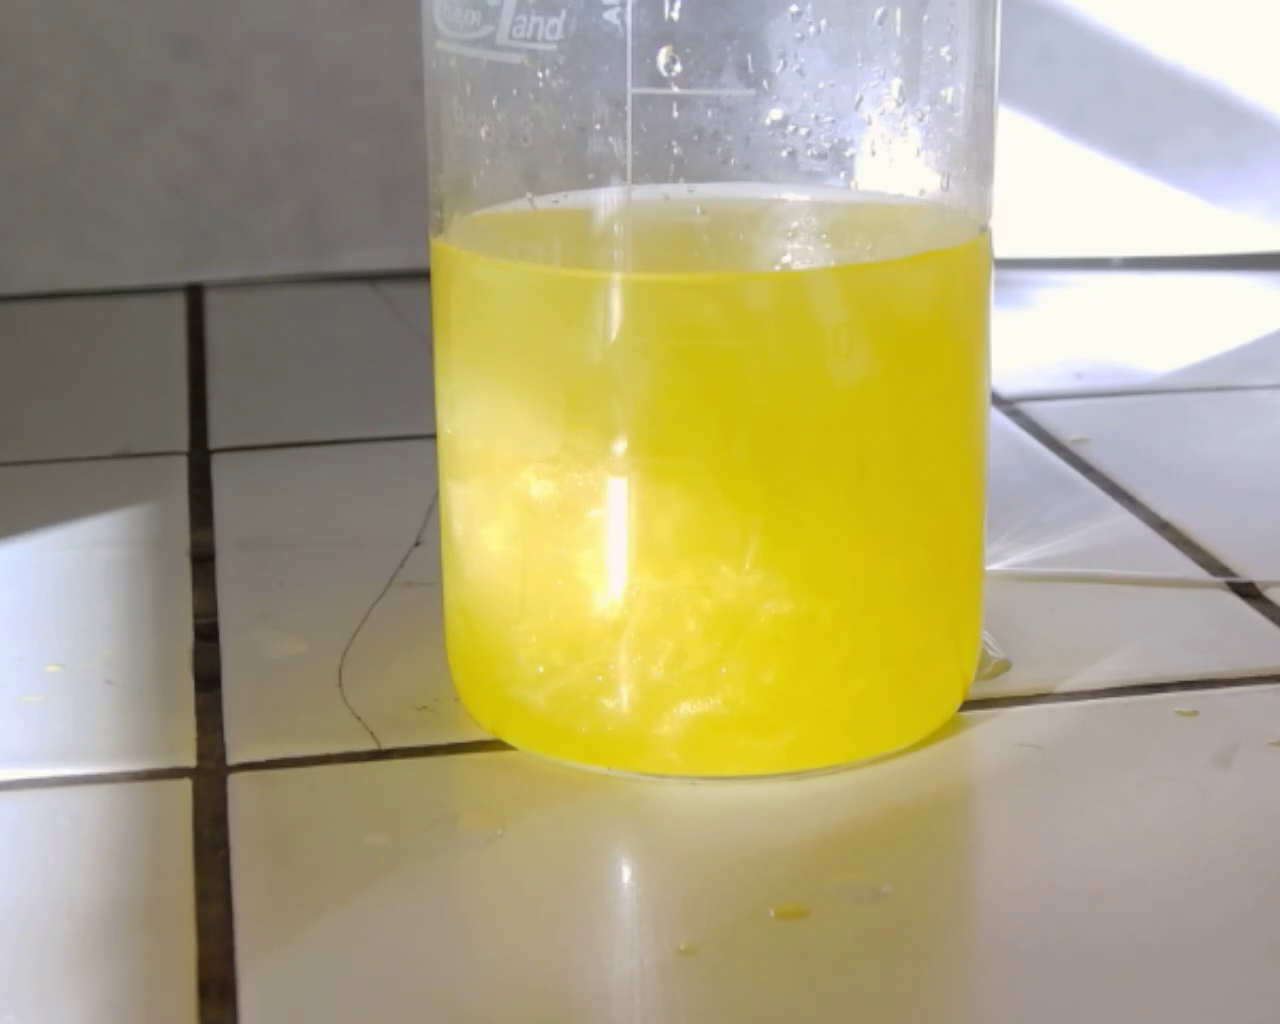
\includegraphics[width=0.45\linewidth]{zlaty_dest.png}
    \caption{Vysrážený zlatý déšť}
\end{figure}

\subsection{Chromatografie na papíře}

\B{Zařazení do výuky}

Tento pokus by mohl být zařazen při výuce chromatografie. Chromatografie je separační metoda, a to z těch běžně vyučovaných asi ta nejneintuitivnější. Pokus názorně vysvětluje její princip, má malé časové i materiální nároky a může být proveden každým žákem samostatně.\\

\hspace{-21pt} \B{Bezpečnost}

Žádné zvláštní bezpečnostní požadavky.\\

\hspace{-21pt} \B{Popis}

Chromatografie je souhrnné označení pro skupinu separačních technik spočívajících v~rozdělování látek mezi dvě nemísitelné fáze - nepohyblivou (stacionární) a~pohyblivou (mobilní). Spolu s~pohybující se mobilní fází je soustavou unášen také vzorek. Dělené složky vzorku (analyty) interagují v~různé míře se stacionární a~mobilní fází. Analyty, které se poutají více ke stacionární fázi, se pohybují pomaleji a~jsou zadržovány déle, než analyty, které se ke stacionární fázi poutají méně. Na základě tohoto principu dochází k~rozdělení složek směsi.

V tomto experimentu je provedena chromatografie v~plošném uspořádání. Jako stacionární fáze je použit filtrační papír, jako mobilní fáze voda nebo ethanol. \newline

\hspace{-21pt} \B{Postup}

\begin{enumerate}
\item Do kádinky nalijeme vrstvu asi 5 mm mobilní fáze (volíme podle typu fixů či obecně látek, které chceme dělit, např. voda, ethanol) a~přikryjeme hodinovým sklem.
\item Vystřihneme obdélník z~filtračního papíru (velký tak, aby se vešel do kádinky) a~tužkou označíme asi 1-2 cm od dolního okraje startovací čáru, na kterou uděláme puntíky fixami asi 1 cm od sebe (nebo naneseme vzorky kapilárou či kapátkem).
\item Vložíme papír s~nanesenými vzorky do kádinky tak, aby se nedotýkal stěn a aby puntíky byly nad hladinou.  Abychom zamezili kontaktu, můžeme horní okraj papíru navléct na špejli nebo drátek (případně papír můžeme přehnout do tvaru obráceného \uv{V} a~nanést vzorky na obě strany). Po vložení papíru opět přikryjeme kádinku hodinovým sklem.
\item Necháme mobilní fázi vzlínat až do vzdálenosti 1 cm pod okraj papíru. Poté papír vyjmeme, označíme tužkou čelo mobilní fáze (= místo, kam vystoupala), papír usušíme a~vyhodnotíme rozdělení barviv.
\item V~případě zájmu můžeme vypočítat retenční faktor Rf pro každou látku. K~tomu potřebujeme určit vzdálenost, kterou urazila látka (střed skvrny) od startovní linie (a), a~vzdálenost, kterou urazila mobilní fáze (b). Rf získáme jako podíl (a)/(b)."
\end{enumerate}

\begin{figure}[h]
    \centering
    \includegraphics[width=0.45\linewidth]{chromatografie.png}
    \caption{Chromatografie dvou barev fixu}
\end{figure}
